\specialchapter{\texorpdfstring{图版 II. \(B_{l}\) 型根系（\(l \geqslant 2\)）}{图版 II. B\_l 型根系 (l >= 2)}}

\begin{enumerate}
\def\labelenumi{(\Roman{enumi})}
\item
  \(V = E = R^{l}\) 。根：\(\pm\varepsilon_{i}, (1\leqslant i\leqslant l), \pm\varepsilon_{i}\pm\varepsilon_{j} (1\leqslant i<j\leqslant l).\) 根的数目：\(n = 2l^{2}\) 。
\item
  基：\(\alpha_{1} = \varepsilon_{1} - \varepsilon_{2},\alpha_{2} = \varepsilon_{2} - \varepsilon_{3},\ldots ,\alpha_{l - 1} = \varepsilon_{l - 1} - \varepsilon_{l},\alpha_{l} = \varepsilon_{l}\) 。正根：
\end{enumerate}

\[
\varepsilon_ {i} = \sum_ {i \leqslant k \leqslant l} \alpha_ {k} (1 \leqslant i \leqslant l),
\]

\[
\varepsilon_ {i} - \varepsilon_ {j} = \sum_ {i \leqslant k <   j} \alpha_ {k} (1 \leqslant i <   j \leqslant l),
\]

\[
\varepsilon_ {i} + \varepsilon_ {j} = \sum_ {i \leqslant k <   j} \alpha_ {k} + 2 \sum_ {j \leqslant k \leqslant l} \alpha_ {k} (1 \leqslant i <   j \leqslant l),
\]

\begin{enumerate}
\def\labelenumi{(\Roman{enumi})}
\setcounter{enumi}{2}
\item
  Coxeter 数：\(h = 2l\) 。
\item
  最高根：
\end{enumerate}

\[
\tilde {\alpha} = \varepsilon_ {1} + \varepsilon_ {2} = \alpha_ {1} + 2 \alpha_ {2} + 2 \alpha_ {3} + \dots + 2 \alpha_ {l}.
\]

有 \(\tilde{\alpha} = 2\omega_{2}\)，当 \(l = 2\) 时；有 \(\tilde{\alpha} = \omega_{2}\)，当 \(l \geqslant 3\) 时。

扩展 Dynkin 图：

当 \(l = 2\) 时：

\pandocbounded{
\includegraphics[keepaspectratio]{images/part002_ab2e3717.jpg}}

当 \(l\geqslant 3\) 时

\pandocbounded{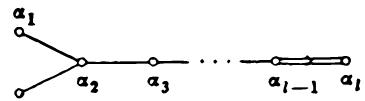
\includegraphics[keepaspectratio]{images/part002_677d35e2.jpg}}

\begin{enumerate}
\def\labelenumi{(\Alph{enumi})}
\setcounter{enumi}{21}
\tightlist
\item
  \(R^{\prime}\) 是向量集
\end{enumerate}

\[
\pm 2 \varepsilon_ {i} (1 \leqslant i \leqslant l), \pm \varepsilon_ {i} \pm \varepsilon_ {j} (1 \leqslant i <   j \leqslant l).
\]

\[
\Phi_ {\mathrm{R}} (x, y) = \frac {(x | y)}{4 l - 2}, \quad \gamma (\mathrm{R}) = (l + 1) (4 l - 2).
\]

\begin{enumerate}
\def\labelenumi{(\Roman{enumi})}
\setcounter{enumi}{5}
\tightlist
\item
  基本权：
\end{enumerate}

\[
\begin{array}{l} \omega_ {i} = \varepsilon_ {1} + \varepsilon_ {2} + \dots + \varepsilon_ {i} (1 \leqslant i <   l) \\ \quad = \alpha_ {1} + 2 \alpha_ {2} + \dots + (i - 1) \alpha_ {i - 1} + i (\alpha_ {i} + \alpha_ {i + 1} + \dots + \alpha_ {l}) \\ \omega_ {l} = \frac {1}{2} (\varepsilon_ {1} + \varepsilon_ {2} + \dots + \varepsilon_ {l}) \\ \quad = \frac {1}{2} (\alpha_ {1} + 2 \alpha_ {2} + \dots + l \alpha_ {l}). \end{array}
\]

\begin{enumerate}
\def\labelenumi{(\Roman{enumi})}
\setcounter{enumi}{6}
\tightlist
\item
  正根之和：
\end{enumerate}

\[
\begin{array}{l} 2 \rho = (2 l - 1) \varepsilon_ {1} + (2 l - 3) \varepsilon_ {2} + \dots + 3 \varepsilon_ {l - 1} + \varepsilon_ {l} \\ = (2 l - 1) \alpha_ {1} + 2 (2 l - 2) \alpha_ {2} + \dots + i (2 l - i) \alpha_ {i} + \dots + l ^ {2} \alpha_ {l}. \end{array}
\]

\begin{enumerate}
\def\labelenumi{(\Roman{enumi})}
\setcounter{enumi}{7}
\tightlist
\item
  \(\mathrm{Q}(\mathrm{R}) = \bigoplus_{i=1}^{l}\mathbf{Z}\varepsilon_i,\mathrm{P}(\mathrm{R}) = \bigoplus_{i=1}^{l}\mathbf{Z}\varepsilon_i + \mathbf{Z}(\frac{1}{2}\sum_{i=1}^{l}\varepsilon_i).\)
\end{enumerate}

\(P(R)/Q(R)\) 同构于 Z/2Z，由 \(\omega_{l}\) 的像生成。连接指标：2。

\begin{enumerate}
\def\labelenumi{(\Roman{enumi})}
\setcounter{enumi}{8}
\item
  指数：1, 3, 5, \ldots, 2l - 1。
\item
  W(R) 是群 \(S_{l}\)（通过对 \(\varepsilon_{i}\) 进行置换作用）与群 \((\mathbf{Z}/2\mathbf{Z})^{l}\)（通过 \(\varepsilon_{i} \mapsto (\pm1)_{i}\varepsilon_{i}\) 作用）的半直积。其阶为 \(2^{l}.l!\)
\item
  A(R) = W(R); \(w_{0} = -1\) .
\item
  \(P(R^{\prime})/Q(R^{\prime})\) 的唯一非平凡元确定扩展 Dynkin 图的唯一非平凡自同构。
\item
  Cartan 矩阵 \((l \times l)\) ：
\end{enumerate}

\[
\left( \begin{array}{c c c c c c c} 2 & - 1 & 0 & 0 & \dots & 0 & 0 \\ - 1 & 2 & - 1 & 0 & \dots & 0 & 0 \\ 0 & - 1 & 2 & - 1 & \dots & 0 & 0 \\ 0 & 0 & - 1 & 2 & \dots & 0 & 0 \\ \vdots & \vdots & \vdots & \vdots & \ddots & \vdots & \vdots \\ 0 & 0 & 0 & 0 & \dots & 2 & - 2 \\ 0 & 0 & 0 & 0 & \dots & - 1 & 2 \end{array} \right)
\]

